\documentclass[../Bitcoin Blink.tex]{subfiles}
\graphicspath{{\subfix{../assets/images/}}}
\begin{document}
\subsection{Forks}
\begin{figure}[H]
\begin{center}
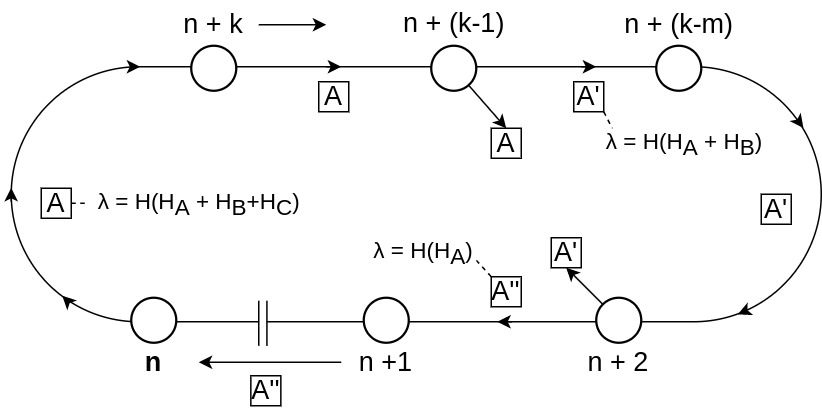
\includegraphics[width=10cm]{intrafork}
\caption{Resolving Forks}
\end{center}
\end{figure}
Confirmed blocks as snips are streamed in a backward ring manner (block$_n$ to block$_{n-1}$...block$_{n+1}$). For each block to prove block time by providing VDF proofs, a set of validators is initialized by ring's size denoting number of blocks and their producers. Intra-block forks arise when ring validators reject snips of a block, this can be resolved by the very next block, providing instant finality to users. Intra-block forks can be minimized by keeping the ring size variable and always lesser than the total number of nodes, a better alternative to sharding. Block size and time are decided on consensus by the block's ring validators bringing a healthy propagation. Bandwidth upgrades are needed for the nodes which initiate the intra-block fork and are punished by the network by not electing them for the upcoming blocks. Each new block will include the previous block's VDF proof which resolves the intra-block forks by selecting the snips and updating the chain using Merkle Chain Roots. During offline activity of ring validators, Inter-block forks arises which can be resolved by attesting VDF Proofs of offline activity and thereby adding negative weights to it.
\end{document}
